\documentclass[../distribution_theory_notes.tex]{subfiles}
\begin{document}
\section{Aula 26 - 25 de Novembro, 2024}
\subsection{Motivações}
\begin{itemize}
	\item Continuação das propriedades da Transformada de Fourier em \(L^{1}\);
	\item Exemplos de transformadas de Fourier;
	\item Transformada de Fourier no espaço de Schwartz.
\end{itemize}

\subsection{Continuação das propriedades de \(\mathcal{F}\) em \(L^{1}\)}
As propriedades (VI) e (VII) possuem uma consequência importante que permite que elas possam ser aplicadas de modo consecutivo em funções de uma determinada classe:

\begin{prop*}[Corolário]
	Seja \(f\in \mathcal{C}^{\infty}\) tal que
	\[
		x^{\alpha }\partial ^{\beta }f\in L^{1}\cap \mathcal{C}_{0},\quad \forall \alpha ,\beta \in \mathbb{Z}_{+}^{n},
	\]
	então \(\xi ^{\alpha }\hat{f}\in \mathcal{C}_{0}^{\infty}\), para todo \(\alpha \in \mathbb{Z}_{+}^{n}\), com
	\[
		\partial _{\xi }^{\beta }\bigl(\xi ^{\alpha }\hat{f}\bigr)
		=(-1)^{|\beta |}(2\pi i)^{|\beta |-|\alpha |}
		\bigl[x^{\beta }(\partial _{x}^{\alpha }f)\bigr]^{\widehat{\; }},
		\quad \forall \alpha ,\beta \in \mathbb{Z}_{+}^{n}.
	\]
\end{prop*}
\begin{proof*}
	Antes de tudo, sendo \(f\in \mathcal{C}^{\infty}\) com \(\partial ^{\alpha }f\in \mathcal{C}_{0}\), para todo \(\alpha \), tem-se que
	\[
		(\partial _{x}^{\alpha }f)^{\widehat{\; }}=(2\pi i\xi )^{\alpha }\hat{f}
	\]
	e \(x^{\beta }f\in L^{1}\), para todo \(\beta \in \mathbb{Z}_{+}^{n}\), dita que \(\hat{f}\in \mathcal{C}^{\infty}\) e
	\[
		\partial _{\xi }^{\beta }\hat{f}=\bigl[(-2\pi i x)^{\beta }f\bigr]^{\widehat{\; }}.
	\]
	Juntando as duas conclusões, \(\xi ^{\alpha }\hat{f}\in \mathcal{C}^{\infty}\), para todo \(\alpha \), o que justifica os cálculos:
	\begin{align*}
		\partial _{\xi }^{\beta }\bigl(\xi ^{\alpha }\hat{f}\bigr)
		&=\partial _{\xi }^{\beta }\bigl[(2\pi i)^{-|\alpha |}(2\pi i\xi )^{\alpha }\hat{f}\bigr]\\
		&=(2\pi i)^{-|\alpha |}\partial _{\xi }^{\beta }\bigl[(2\pi i\xi )^{\alpha }\hat{f}\bigr]\\
		&=(2\pi i)^{-|\alpha |}\partial _{\xi }^{\beta }\bigl[\partial _{x}^{\alpha }f\bigr]^{\widehat{\; }}\\
		&=(2\pi i)^{-|\alpha |}\bigl[(-2\pi i x)^{\beta }(\partial _{x}^{\alpha }f)\bigr]^{\widehat{\; }}\\
		&=(-1)^{|\beta |}(2\pi i)^{|\beta |-|\alpha |}\bigl[x^{\beta }(\partial _{x}^{\alpha }f)\bigr]^{\widehat{\; }}.
	\end{align*}
	\qedsymbol
\end{proof*}

Mais um fato relacionado a funções integráveis, o qual já sugere como definir \(\mathcal{F}\) em distribuições, deve ser destacado:
\[
\text{(VIII)}\qquad \int_{\mathbb{R}^{n}}\hat{f}(\xi )g(\xi )\,\mathrm{d}\xi
=\int_{\mathbb{R}^{n}}f(x)\hat{g}(x)\,\mathrm{d}x.
\]
\begin{proof*}
	Surpreende o fato de que essa propriedade não apresenta dificuldade alguma para ser demonstrada, dado que se conheça o Teorema de Fubini:
	\begin{align*}
		\int_{\mathbb{R}^{n}}\hat{f}(\xi )g(\xi )\,\mathrm{d}\xi
		&=\int_{\mathbb{R}^{n}}\biggl[\int_{\mathbb{R}^{n}}e^{-2\pi i x\cdot \xi }f(x)\,\mathrm{d}x\biggr]g(\xi )\,\mathrm{d}\xi\\
		&=\int_{\mathbb{R}^{n}}f(x)\biggl[\int_{\mathbb{R}^{n}}e^{-2\pi i x\cdot \xi }g(\xi )\,\mathrm{d}\xi\biggr]\,\mathrm{d}x\\
		&=\int_{\mathbb{R}^{n}}f(x)\hat{g}(x)\,\mathrm{d}x.
	\end{align*}
	O Teorema de Fubini pode ser aplicado porque
	\[
		\mathbb{R}^{n}\times \mathbb{R}^{n}\longrightarrow \mathbb{C},\qquad (x,\xi )\longmapsto f(x)g(\xi )
	\]
	é integrável em \(\mathbb{R}^{n}\times \mathbb{R}^{n}\), segundo \(\mathrm{d}x\,\mathrm{d}\xi\), sempre que \(f,g\in L^{1}\). \qedsymbol
\end{proof*}

\subsection{A Transformada de Fourier}
Duas das principais ferramentas (ou operações) de trabalho da Fourier são a ``convolução'' e a ``Transformada de Fourier'', sendo essa última a definitiva para a consolidação da teoria das Distribuições (em detrimento de outras baseadas em medidas e técnicas parecidas).

A transformada é, na A.F., estudada em dois contextos (ou níveis):
\begin{itemize}
	\item[(i)] o das funções periódicas, identificadas com funções em ``toros'' \(\mathbb{T}^{n}\);
	\item[(ii)] o das funções integráveis em \(\mathbb{R}^{n}\).
\end{itemize}
No nível (i), ela aparece como mecanismo necessário para se resolverem PVI e de contorno para EDP do Calor numa faixa do tipo \([0,\ell ]\times [0,\infty )\), sendo \(\ell >0\) o comprimento de um fio (ou barra ``fina'') submetida a uma temperatura inicial \(f:[0,\ell ]\rightarrow \mathbb{R}\), e cuja ``difusão'' do calor ao longo da barra se deseja investigar com o passar do tempo \(t>0\). Aqui, a solução é procurada como tendo a forma
\[
	u(x,t)=\varphi (x)T(t),
\]
e, quase que exclusivamente baseando-se em métodos de Análise Funcional em Espaços de Hilbert, uma teoria muito fértil é desenvolvida.

Nem tudo o que é conseguido em (i) pode ser imediatamente deduzido em (ii). Um exemplo disso é que os casos desenvolvem-se ``ao contrário'': em (i), começa-se em \(L^{2}\) e passa-se a \(L^{1}\); já em (ii), começamos com \(L^{1}\) e passamos para \(L^{2}\), baseados fortemente em fatos da Teoria de Medida.

Outro elemento importante é que os ``núcleos'' que produzem as soluções no espaço têm a mesma forma:
\begin{itemize}
	\item[(i)] tem
	\[
		K(x,t)=\sum_{n=-\infty }^{\infty }e^{-4\pi ^{2}n^{2}t}P_{n},
	\]
	com \(P_{n}\) a projeção sobre o auto-espaço \([e^{2\pi i n x}]\);
	\item[(ii)] tem
	\[
		E(x,t)=H(t)\frac{1}{(4\pi t)^{n/2}}e^{-\frac{|x|^{2}}{4t}},\qquad (x,t)\in \mathbb{R}^{n}\times \mathbb{R}.
	\]
\end{itemize}

Hoje, continuaremos com o estabelecimento das propriedades da \(\mathcal{F}\), até o ponto que sugere como estendê-la para uma classe de distribuições (as Temperadas), o que se faz restringindo, a princípio, a análise ao espaço \(\mathcal{S}\). Além disso, calcularemos, explicitamente, algumas transformadas importantes para o desenvolvimento dos métodos.

\subsection{Exemplos}
\begin{example}
	\textbf{(1)} Seja \(a>0\) e consideremos \(f=\chi _{[-a,a]}\), a característica do intervalo \([-a,a]\). Claramente, \(f\in L^{1}(\mathbb{R})\) e podemos calcular:
	\[
		\hat{f}(0)=\int_{\mathbb{R}}e^{-2\pi i x\cdot 0}\chi _{[-a,a]}(x)\,\mathrm{d}x
		=\int_{-a}^{a}\mathrm{d}x=2a.
	\]
	Se \(\xi \neq 0\),
	\begin{align*}
		\hat{f}(\xi )
		&=\int_{\mathbb{R}}e^{-2\pi i x\xi }\chi _{[-a,a]}(x)\,\mathrm{d}x
		=\int_{-a}^{a}e^{-2\pi i x\xi }\,\mathrm{d}x\\
		&=\left.\frac{e^{-2\pi i x\xi }}{-2\pi i\xi }\right|_{-a}^{a}
		=-\frac{1}{2\pi i\xi }\bigl[e^{-2\pi i a\xi }-e^{2\pi i a\xi }\bigr]\\
		&=\frac{\sin (2\pi a\xi )}{\pi \xi }.
	\end{align*}
	Aqui, foi usada a identidade \(z-\overline{z}=2i\operatorname{Im}(z)\). Assim, para todo \(\xi \in \mathbb{R}\),
	\[
		\hat{f}(\xi )=\frac{\sin (2\pi a\xi )}{\pi \xi },
	\]
	que admite extensão analítica a todo o \(\mathbb{C}\):
	\[
		U(\zeta )=\frac{\sin (2\pi a\zeta )}{\pi \zeta },\qquad \zeta \in \mathbb{C}.
	\]
	\begin{figure}[H]
		\begin{center}
			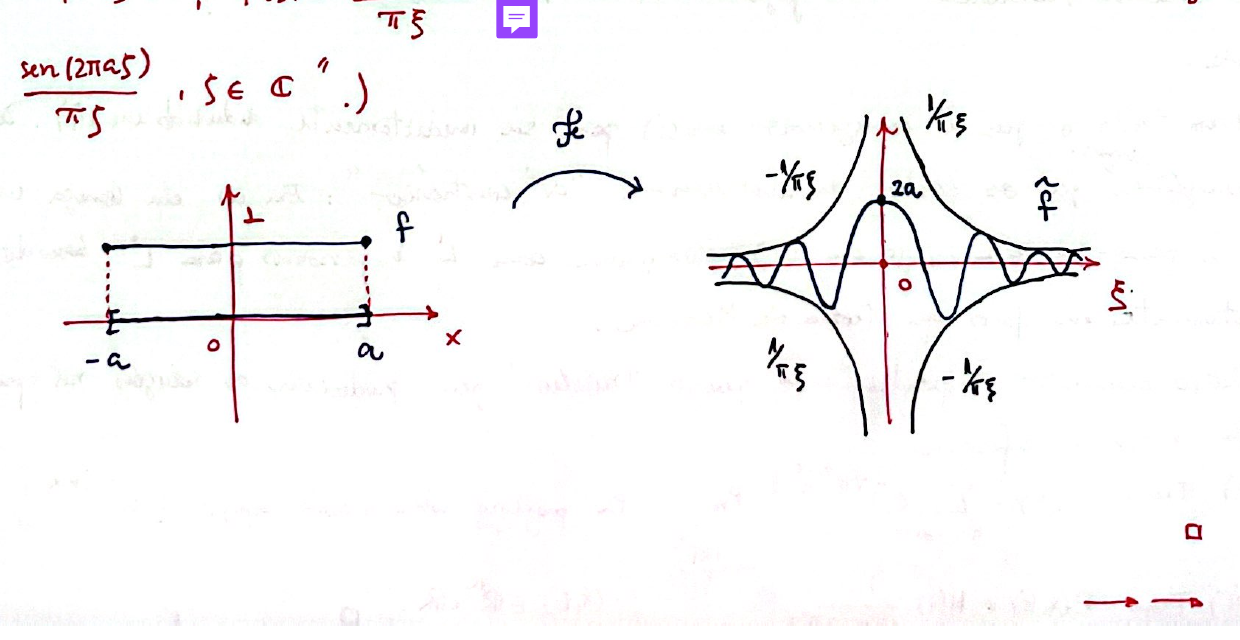
\includegraphics[height=0.32\textheight, width=0.85\textwidth, keepaspectratio]{./Images/fourier_indicator_26.png}
		\end{center}
	\end{figure}
\end{example}

\begin{example}
	\textbf{(2)} Se \(a>0\) e pusermos
	\[
		f_{a}(x)=e^{-a|x|},\qquad x\in \mathbb{R},
	\]
	é claro que \(f_{a}\in L^{1}(\mathbb{R})\) e, assim, existe \(\hat{f}_{a}\). Dado \(\xi \in \mathbb{R}\),
	\[
		\hat{f}_{a}(\xi )=\int_{\mathbb{R}}e^{-2\pi i x\xi }e^{-a|x|}\,\mathrm{d}x
		=\biggl(\int_{-\infty }^{0}+\int_{0}^{\infty }\biggr)e^{-2\pi i x\xi }e^{-a|x|}\,\mathrm{d}x,
	\]
	e calculamos separadamente:
	\begin{align*}
		\int_{0}^{\infty }e^{-2\pi i x\xi }e^{-ax}\,\mathrm{d}x
		&=\lim_{N\to \infty }\int_{0}^{N}e^{-x(2\pi i\xi +a)}\,\mathrm{d}x
		=\lim_{N\to \infty }\left.\frac{e^{-x(2\pi i\xi +a)}}{-(2\pi i\xi +a)}\right|_{0}^{N}
		=\frac{1}{2\pi i\xi +a},\\
		\int_{-\infty }^{0}e^{-2\pi i x\xi }e^{ax}\,\mathrm{d}x
		&=\lim_{N\to \infty }\int_{-N}^{0}e^{x(a-2\pi i\xi )}\,\mathrm{d}x
		=\lim_{N\to \infty }\left.\frac{e^{x(a-2\pi i\xi )}}{a-2\pi i\xi }\right|_{-N}^{0}
		=\frac{1}{a-2\pi i\xi }.
	\end{align*}
	Donde
	\[
		\hat{f}_{a}(\xi )=\frac{1}{a+2\pi i\xi }+\frac{1}{a-2\pi i\xi }
		=\frac{2a}{a^{2}+4\pi ^{2}\xi ^{2}},\qquad \xi \in \mathbb{R}.
	\]
	\begin{figure}[H]
		\begin{center}
			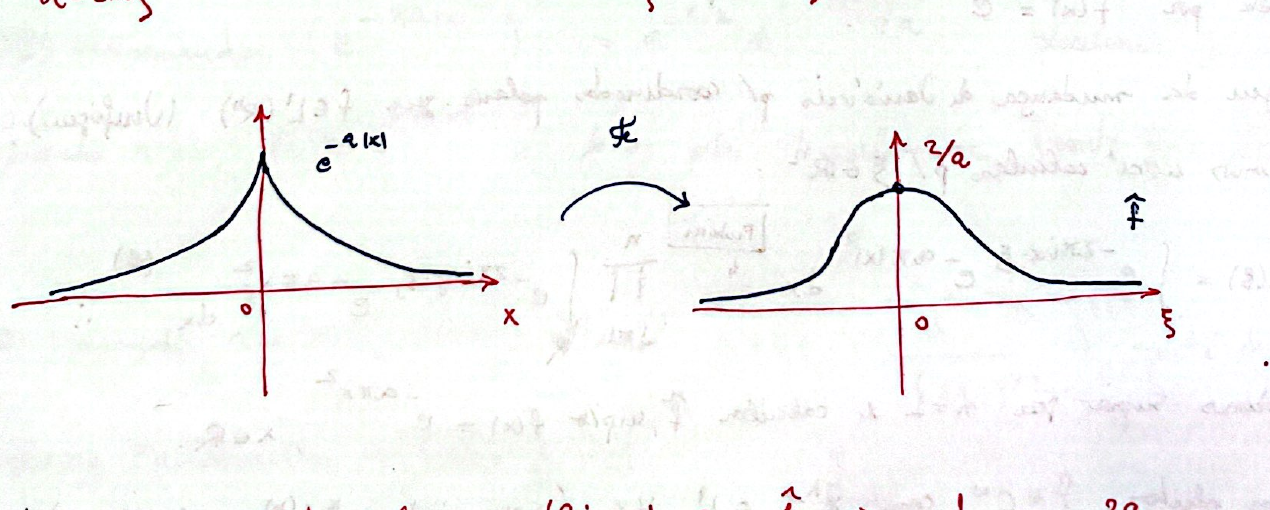
\includegraphics[height=0.30\textheight, width=0.85\textwidth, keepaspectratio]{./Images/fourier_exponential_26.png}
		\end{center}
	\end{figure}

	\textbf{Obs. (1)} Escolhendo valores específicos de \(a\):
	\[
		\hat{f}_{a}(\xi )=\frac{1}{4\pi ^{2}}\frac{2a}{\left(\frac{a^{2}}{4\pi ^{2}}\right)+\xi ^{2}}.
	\]
	Dado \(t>0\), \(a=2\pi t\), então
	\[
		\hat{f}_{a}(\xi )=\frac{t}{\pi (t^{2}+\xi ^{2})}.
	\]
	Note que \(t>0\) é variável, definindo assim uma função de duas variáveis:
	\[
		P(\xi ,t)=\frac{t}{\pi (t^{2}+\xi ^{2})},\qquad \xi \in \mathbb{R},\; t>0,
	\]
	chamado o Núcleo de Poisson em \(\mathbb{R}\times \mathbb{R}^{+}\), definido no semiplano \(\mathbb{R}_{+}^{2}\).

	Note que
	\[
		\forall \xi ,\qquad \lim_{t\to 0^{+}}P(\xi ,t)=\infty
	\]
	e
	\begin{align*}
		\int_{\mathbb{R}}P(t,\xi )\,\mathrm{d}\xi
		&=\frac{t}{\pi }\int_{-\infty }^{\infty }\frac{1}{t^{2}+\xi ^{2}}\,\mathrm{d}\xi\\
		&=\frac{1}{t\pi }\int_{-\infty }^{\infty }\frac{1}{1+(\xi /t)^{2}}\,\mathrm{d}\xi
		=\left.\frac{1}{\pi }\operatorname{arctg}(u)\right|_{-\infty }^{\infty }=1.
	\end{align*}

	\textbf{(2)} O cálculo realizado em (ii), por si só, é interessante, pois, tomando \(g_{a}=\chi _{(0,\infty )}f_{a}\), vimos que
	\[
		\hat{g}_{a}(\xi )=\frac{1}{a+2\pi i\xi },
	\]
	e, escolhendo \(a=2\pi t\), como antes, obtemos
	\[
		\hat{g}_{a}(\xi )=\frac{1}{2\pi }\frac{1}{t+i\xi }.
	\]
	Portanto,
	\[
		F(t,\xi )=\hat{g}_{2\pi t}(\xi )=\frac{1}{2\pi z},\qquad z=t+i\xi \in \mathbb{C},\; t>0.
	\]
	Analogamente, \(h_{a}=\chi _{(-\infty ,0)}f_{a}\) daria
	\[
		G(t,\xi )=\hat{h}_{2\pi t}(\xi )=\frac{1}{2\pi \overline{z}},\qquad z=t+i\xi ,\; t>0.
	\]
\end{example}

\begin{example}
	\textbf{(3) Importantíssimo:} Agora em \(\mathbb{R}^{n}\). Seja ainda \(a>0\) e consideremos \(f:\mathbb{R}^{n}\rightarrow \mathbb{R}\) dada por
	\[
		f(x)=e^{-a\pi |x|^{2}}.
	\]
	Segue da mudança de variáveis para coordenadas polares que \(f\in L^{1}(\mathbb{R}^{n})\) (verifique), podendo então calcular, para \(\xi \in \mathbb{R}^{n}\),
	\begin{align*}
		\hat{f}(\xi )
		&=\int_{\mathbb{R}^{n}}e^{-2\pi i x\cdot \xi }e^{-a\pi |x|^{2}}\,\mathrm{d}x\\
		&=\prod_{j=1}^{n}\int_{\mathbb{R}}e^{-2\pi i x_{j}\xi _{j}}e^{-a\pi x_{j}^{2}}\,\mathrm{d}x_{j}. \qquad (\#)
	\end{align*}
	Podemos supor que \(n=1\) e calcular \(\hat{f}\), sendo
	\[
		f(x)=e^{-a\pi x^{2}},\qquad x\in \mathbb{R}.
	\]
	Com efeito, \(f\in \mathcal{C}^{\infty}\) com \(x^{k}f\in L^{1}\), para todo \(k\) (mais ainda, \(x^{k}f^{(m)}\in L^{1}\), para todo \(m,k\)), e \(f^{(m)}\in \mathcal{C}_{0}\), para todo \(m\) (\(x^{k}f^{(m)}\in \mathcal{C}_{0}\), etc.). Portanto, \(\hat{f}\in \mathcal{C}^{\infty}\) e, aplicando as propriedades (VI) e (VII) da Aula 25, podemos escrever:
	\begin{align*}
		\frac{\mathrm{d}f}{\mathrm{d}x}=-2a\pi x f
		&\Rightarrow 2\pi i\xi \hat{f}=\biggl(\frac{\mathrm{d}f}{\mathrm{d}x}\biggr)^{\widehat{\; }}
		=(-2\pi a x f)^{\widehat{\; }}
		=\frac{a}{i}(-2\pi i x f)^{\widehat{\; }}\\
		&=\frac{a}{i}\frac{\mathrm{d}\hat{f}}{\mathrm{d}\xi }.
	\end{align*}
	Logo,
	\[
		\frac{\mathrm{d}\hat{f}}{\mathrm{d}\xi }=-\frac{2\pi }{a}\xi \hat{f}
		\Rightarrow \frac{\mathrm{d}\hat{f}}{\mathrm{d}\xi }+\frac{2\pi }{a}\xi \hat{f}=0
		\Rightarrow \frac{\mathrm{d}}{\mathrm{d}\xi }\bigl(e^{\frac{\pi }{a}\xi ^{2}}\hat{f}\bigr)=0.
	\]
	Logo, existe \(c\in \mathbb{C}\) tal que
	\[
		e^{\frac{\pi }{a}\xi ^{2}}\hat{f}(\xi )=c,\qquad \forall \xi \in \mathbb{R},
	\]
	isto é,
	\[
		\hat{f}(\xi )=ce^{-\frac{\pi }{a}\xi ^{2}}.
	\]
	É possível calcular \(c\) explicitamente, porque
	\begin{align*}
		c=\hat{f}(0)=\int_{\mathbb{R}}e^{-a\pi x^{2}}\,\mathrm{d}x
		&=\int_{\mathbb{R}}e^{-u^{2}}\frac{\mathrm{d}u}{\sqrt{\pi a}}\\
		&=\frac{1}{\sqrt{\pi a}}\int_{\mathbb{R}}e^{-u^{2}}\,\mathrm{d}u
		=\frac{1}{\sqrt{a}},
	\end{align*}
	pois \(\int_{\mathbb{R}}e^{-u^{2}}\,\mathrm{d}u=\sqrt{\pi}\), conforme o Cálculo nos ensina. Assim,
	\[
		\hat{f}(\xi )=\frac{1}{\sqrt{a}}e^{-\frac{\pi }{a}\xi ^{2}}.
	\]
	Finalmente, por (\#), o caso \(n\)-dimensional fica:
	\[
		\hat{f}(\xi )=\prod_{j=1}^{n}\biggl(\frac{1}{\sqrt{a}}e^{-\frac{\pi }{a}\xi _{j}^{2}}\biggr)
		=\frac{1}{a^{n/2}}e^{-\frac{\pi }{a}|\xi |^{2}}
		=a^{-n/2}e^{-\pi |\xi |^{2}/a}.
	\]

	\textbf{Obs. (1)} Escolhendo \(a=1\),
	\[
		\bigl(e^{-\pi a|x|^{2}}\bigr)^{\widehat{\; }}=a^{-n/2}e^{-\pi |\xi |^{2}/a},
	\]
	percebemos que, quando \(a=1\), \(f(x)=e^{-\pi |x|^{2}}\) é fixa pela transformada, isto é, um ponto fixo: \(\mathcal{F}(f)=f\).

	\textbf{(2)} Tomando \(a=4\pi t\), \(t>0\), obtemos
	\[
		E(\xi ,t)=\frac{e^{-\frac{|\xi |^{2}}{4t}}}{(4\pi t)^{n/2}},\qquad \xi \in \mathbb{R}^{n},
	\]
	``parte'' da solução Fundamental de
	\[
		P(D)=\frac{\partial }{\partial t}-\Delta .
	\]
\end{example}

\subsection{Transformada de Fourier em \(\mathcal{S}\)}
Queremos agora estudar de fato o comportamento da \(\mathcal{F}\) nas funções de \(\mathcal{S}\) (o espaço de Schwartz: funções de decaimento rápido). O primeiro passo consiste em estabelecer uma (ou outra) caracterização das funções de \(\mathcal{S}\).

\begin{lemma*}
	Seja \(f\in \mathcal{C}^{\infty}(\mathbb{R}^{n})\). São equivalentes:
	\begin{itemize}
		\item[(i)] \(f\in \mathcal{S}\);
		\item[(ii)] \(x^{\alpha }\partial ^{\beta }f\in L^{\infty}\), para todo \(\alpha ,\beta \in \mathbb{Z}_{+}^{n}\);
		\item[(iii)] \(\partial ^{\beta }(x^{\alpha }f)\in L^{\infty}\), para todo \(\alpha ,\beta \in \mathbb{Z}_{+}^{n}\).
	\end{itemize}
\end{lemma*}
\begin{tcolorbox}[
		skin=enhanced,
		title=Observação,
		fonttitle=\bfseries,
		colframe=black,
		colbacktitle=cyan!75!white,
		colback=cyan!15,
		colbacklower=black,
		coltitle=black,
		drop fuzzy shadow
	]
	Mais precisamente, esse lema estabelece que as seminormas
	\begin{align*}
		\text{(i)}\quad &\|f\|_{(N,\alpha )}=\sup_{x\in \mathbb{R}^{n}}(1+|x|)^{N}|\partial ^{\alpha }f(x)|,\\
		\text{(ii)}\quad &P_{(\alpha ,\beta )}(f)=\sup_{x\in \mathbb{R}^{n}}|x^{\alpha }\partial ^{\beta }f(x)|,\\
		\text{(iii)}\quad &q_{(\alpha ,\beta )}(f)=\sup_{x\in \mathbb{R}^{n}}|\partial ^{\beta }(x^{\alpha }f)(x)|
	\end{align*}
	definem a mesma topologia em \(\mathcal{S}\).
\end{tcolorbox}

\begin{proof*}
	\textbf{(i) \(\Rightarrow\) (ii).} Dados \(\alpha ,\beta \in \mathbb{Z}_{+}^{n}\), tem-se que \(|x^{\alpha }|\leq |x|^{|\alpha |}\); logo,
	\[
		|x^{\alpha }\partial ^{\beta }f(x)|
		\leq |x|^{|\alpha |}|\partial ^{\beta }f(x)|
		\leq (1+|x|)^{|\alpha |}|\partial ^{\beta }f(x)|
		\leq \|f\|_{(|\alpha |,\beta )}<\infty ,\qquad \forall x\in \mathbb{R}^{n}.
	\]

	\textbf{(ii) \(\Rightarrow\) (i).} Começamos observando que a função \(\varphi (t)=t^{N}\), \(t\geq 0\), é convexa para todo \(N\in \mathbb{N}\). Portanto,
	\[
		\varphi \biggl(\frac{t+s}{2}\biggr)\leq \frac{1}{2}\varphi (t)+\frac{1}{2}\varphi (s),\qquad \forall t,s\geq 0,
	\]
	logo
	\[
		(1+|x|)^{N}\leq 2^{N-1}(1+|x|^{N}),\qquad \forall x\in \mathbb{R}^{n}.
	\]
	Agora, estudamos a função, um polinômio homogêneo de grau \(N\),
	\[
		h(x)=\sum_{j=1}^{n}|x_{j}|^{N},
	\]
	a qual é positiva sobre \(S^{n-1}\) (suponha \(n\geq 2\) aqui). Existe
	\[
		\delta =\inf_{|x|=1}h(x)>0.
	\]
	Consequentemente, para todo \(x\neq 0\),
	\[
		\delta \leq h\biggl(\frac{x}{|x|}\biggr)
		=\frac{1}{|x|^{N}}\sum_{j=1}^{n}|x_{j}|^{N},
	\]
	donde
	\[
		\delta |x|^{N}\leq \sum_{j=1}^{n}|x_{j}|^{N}.
	\]
	Como \(h(0)=0\),
	\[
		\delta |x|^{N}\leq \sum_{j=1}^{n}|x_{j}|^{N},\qquad \forall x\in \mathbb{R}^{n},
	\]
	notando que \(\delta \) depende de \(N\).

	Perceba também que
	\[
		|x_{j}|^{N}=|x_{j}^{N}|=|x^{Ne_{j}}|=|x^{\alpha }|,
	\]
	sendo \(\alpha =Ne_{j}=(0,\dotsc ,0,N,0,\dotsc ,0)\). Com isso, concluímos que, para todo \(N\) e \(\beta \in \mathbb{Z}_{+}^{n}\),
	\begin{align*}
		(1+|x|)^{N}|\partial ^{\beta }f(x)|
		&\leq 2^{N-1}|\partial ^{\beta }f(x)|+2^{N-1}|x|^{N}|\partial ^{\beta }f(x)|\\
		&\leq 2^{N-1}|\partial ^{\beta }f(x)|+\frac{2^{N-1}}{\delta }\sum_{j=1}^{n}|x_{j}|^{N}|\partial ^{\beta }f(x)|\\
		&\leq C_{N}\biggl(|x^{0}||\partial ^{\beta }f(x)|+\sum_{j=1}^{n}|x^{Ne_{j}}||\partial ^{\beta }f(x)|\biggr)\\
		&\leq C_{N}\sum_{|\alpha |=0}^{N}P_{(\alpha ,\beta )}(f)<\infty ,
	\end{align*}
	onde
	\[
		C_{N}=\max \biggl\{2^{N-1},\frac{2^{N-1}}{\delta }\biggr\}>0
	\]
	e
	\[
		P_{(\alpha ,\beta )}(f)=\sup_{x\in \mathbb{R}^{n}}|x^{\alpha }\partial ^{\beta }f(x)|.
	\]
	Como \(x\in \mathbb{R}^{n}\) foi arbitrário,
	\[
		\|f\|_{(N,\beta )}\leq C_{N}\sum_{|\alpha |=0}^{N}P_{(\alpha ,\beta )}(f)<\infty ,
	\]
	e (ii) implica (i).

	\textbf{(ii) \(\Rightarrow\) (iii).} Vamos escrever
	\[
		q_{(\alpha ,\beta )}(f)=\sup_{x\in \mathbb{R}^{n}}|\partial ^{\beta }(x^{\alpha }f)(x)|,
		\qquad \alpha ,\beta \in \mathbb{Z}_{+}^{n}.
	\]
	Dados \(\alpha ,\beta \in \mathbb{Z}_{+}^{n}\), pela Regra de Leibniz deve valer
	\[
		\partial ^{\beta }(x^{\alpha }f)
		=\sum_{\gamma +\delta =\beta }\frac{\beta !}{\gamma !\delta !}(\partial ^{\gamma }x^{\alpha })(\partial ^{\delta }f). \qquad (\#)
	\]
	Como cada derivada \(\partial ^{\gamma }x^{\alpha }\) é da forma
	\[
		\frac{\alpha !}{(\alpha -\gamma )!}x^{\alpha -\gamma },\qquad \gamma _{j}\leq \alpha _{j},\; \forall j,
	\]
	ou é nula, se algum \(\gamma _{j}>\alpha _{j}\), temos
	\[
		\partial ^{\beta }(x^{\alpha }f)
		=\sum_{\substack{\gamma +\delta =\beta \\ \gamma \leq \alpha }}
		\frac{\beta !}{\gamma !\delta !}\frac{\alpha !}{(\alpha -\gamma )!}
		x^{\alpha -\gamma }(\partial ^{\delta }f).
	\]
	Aqui, \(\gamma \leq \alpha \) significa \(\gamma _{j}\leq \alpha _{j}\), para todo \(j=1,2,\dotsc ,n\).

	Daí, se \(C=C_{(\alpha ,\beta )}=\beta !\alpha !\), que é maior do que todas as constantes acima, para todo \(x\in \mathbb{R}^{n}\),
	\[
		|\partial ^{\beta }(x^{\alpha }f)(x)|
		\leq C\sum_{|\gamma |\leq |\alpha |+|\beta |}|x^{\gamma }\partial ^{\gamma }f(x)|
		\leq C\sum_{|\gamma |\leq |\alpha |+|\beta |}P_{(\gamma ,\gamma )}(f)<\infty .
	\]
	Logo,
	\[
		q_{(\alpha ,\beta )}(f)\leq C\sum_{|\gamma |\leq |\alpha |+|\beta |}P_{(\gamma ,\gamma )}(f),
	\]
	provando que, de fato, (ii) implica (iii).

	\textbf{(iii) \(\Rightarrow\) (ii).} Começamos escrevendo (\#) assim:
	\begin{align*}
		\partial ^{\beta }(x^{\alpha }f)
		&=x^{\alpha }\partial ^{\beta }f
		+\sum_{\substack{\gamma +\delta =\beta \\ \gamma \neq 0}}
		\frac{\beta !}{\gamma !\delta !}(\partial ^{\gamma }x^{\alpha })(\partial ^{\delta }f)\\
		&=x^{\alpha }\partial ^{\beta }f
		+\sum_{\substack{\gamma +\delta =\beta \\ 0\neq \gamma \leq \alpha }}
		\frac{\beta !}{\gamma !\delta !}\frac{\alpha !}{(\alpha -\gamma )!}x^{\alpha -\gamma }\partial ^{\delta }f,
	\end{align*}
	donde
	\[
		x^{\alpha }\partial ^{\beta }f
		=\partial ^{\beta }(x^{\alpha }f)
		-\sum_{\substack{\gamma +\delta =\beta \\ 0\neq \gamma \leq \alpha }}
		\frac{\beta !}{\gamma !\delta !}\frac{\alpha !}{(\alpha -\gamma )!}x^{\alpha -\gamma }\partial ^{\delta }f. \qquad (\#\#)
	\]
	Observemos que essa providência escreve a soma acima como combinação linear de funções do tipo \(x^{\eta }\partial ^{\delta }f\), nas quais \(|\eta |<|\alpha |\), pois \(\gamma \neq 0\) implica \(|\alpha -\gamma |=|\alpha |-|\gamma |<|\alpha |\), e \(|\delta |<|\beta |\), porque \(\gamma \neq 0\) implica \(\delta \neq \beta \), com \(\delta =\beta -\gamma \), portanto \(|\delta |<|\beta |\). É isso que nos permite usar indução para demonstrar a afirmação.

	Com efeito, suponhamos que
	\[
		q_{(\alpha ,\beta )}(f)<\infty ,\qquad \forall \alpha ,\beta \in \mathbb{Z}_{+}^{n},
	\]
	implique \(P_{(\eta ,\delta )}(f)<\infty \) quando \(|\eta |\leq m\) e \(|\delta |\leq k\), para certos \(m,k\in \mathbb{N}\), e mostramos que isso também ocorre quando \(|\eta |=m+1\) ou \(|\delta |=k+1\). Note que
	\[
		P_{(\alpha ,0)}(f)=q_{(\alpha ,0)}(f)\quad \text{e}\quad P_{(0,\beta )}(f)=q_{(0,\beta )}(f),\qquad \forall \alpha ,\beta .
	\]
	Isso decorre imediatamente de (\#\#), porque, se \(|\alpha |=m+1\) ou \(|\beta |=k+1\), então
	\[
		P_{(\alpha -\gamma ,\delta )}(f)<\infty ,
	\]
	pois \(0\neq \gamma \leq \alpha \) implica \(|\alpha -\gamma |<|\alpha |=m+1\), portanto \(|\alpha -\gamma |\leq m\), e
	\[
		|\delta |=|\beta |-|\gamma |<|\beta |=k+1,
	\]
	logo \(|\delta |\leq k\), e usamos a hipótese de indução. A parcela isolada é limitada por \(q_{(\alpha ,\beta )}(f)\), que é finita por hipótese, donde
	\[
		P_{(\alpha ,\beta )}(f)
		\leq q_{(\alpha ,\beta )}(f)
		+C\sum_{\substack{|\eta |\leq m\\|\delta |\leq k}}P_{(\eta ,\delta )}(f),
	\]
	o que completa a prova. \qedsymbol
\end{proof*}

Usando as propriedades e o lema anterior, podemos mostrar que \(\mathcal{F}\) aplica \(\mathcal{S}\) em si mesmo continuamente. Antes, uma observação:

\begin{tcolorbox}[
		skin=enhanced,
		title=Observação 1,
		fonttitle=\bfseries,
		colframe=black,
		colbacktitle=cyan!75!white,
		colback=cyan!15,
		colbacklower=black,
		coltitle=black,
		drop fuzzy shadow
	]
	Pela M.V. para coordenadas polares, dado \(N\in \mathbb{N}\), temos que
	\begin{align*}
		\int_{\mathbb{R}^{n}}(1+|x|)^{-N}\,\mathrm{d}x
		&=\sigma (S^{n-1})\int_{0}^{\infty }(1+r)^{-N}r^{n-1}\,\mathrm{d}r\\
		&=\sigma _{n}\int_{0}^{1}(1+r)^{-N}r^{n-1}\,\mathrm{d}r
		+\sigma _{n}\int_{1}^{\infty }(1+r)^{-N}r^{n-1}\,\mathrm{d}r\\
		&\leq \sigma _{n}\int_{0}^{1}r^{n-1}\,\mathrm{d}r
		+\sigma _{n}\int_{1}^{\infty }r^{n-N-1}\,\mathrm{d}r.
	\end{align*}
	A primeira parcela é finita, independentemente de \(N\) (ou \(n\)), e a segunda é finita sempre que
	\[
		n-N-1<-1\Longleftrightarrow N>n.
	\]
	Portanto,
	\[
		(1+|x|)^{-N}\in L^{1},\qquad \text{se }N>n.
	\]
	Mais geralmente,
	\[
		(1+|x|)^{-N}\in L^{p},\qquad \text{se }N>\frac{n}{p}.
	\]
\end{tcolorbox}

\begin{tcolorbox}[
		skin=enhanced,
		title=Observação 2,
		fonttitle=\bfseries,
		colframe=black,
		colbacktitle=cyan!75!white,
		colback=cyan!15,
		colbacklower=black,
		coltitle=black,
		drop fuzzy shadow
	]
	A observação anterior garante que
	\[
		\mathcal{S}\hookrightarrow L^{p},\qquad \forall 1\leq p\leq \infty .
	\]
	Com efeito, se \(f\in \mathcal{S}\), então
	\begin{align*}
		\int_{\mathbb{R}^{n}}|f(x)|^{p}\,\mathrm{d}x
		&=\int_{\mathbb{R}^{n}}(1+|x|)^{-Np}\bigl[(1+|x|)^{Np}|f(x)|^{p}\bigr] \,\mathrm{d}x\\
		&\leq \|f\|_{(N,0)}^{p}\int_{\mathbb{R}^{n}}(1+|x|)^{-Np}\,\mathrm{d}x.
	\end{align*}
	Tomando \(N>n/p\), para que essa integral seja finita, obtém-se
	\[
		\|f\|_{L^{p}}\leq C_{p,n}\|f\|_{(N,0)}.
	\]
\end{tcolorbox}

\begin{theorem*}
	\(\mathcal{F}\) aplica \(\mathcal{S}\) em si mesmo continuamente, isto é, \(\mathcal{S}\) é invariante por \(\mathcal{F}\).
\end{theorem*}
\begin{proof*}
	Com efeito, se \(f\in \mathcal{S}\), então
	\[
		x^{\alpha }\partial ^{\beta }f\in L^{1}\cap \mathcal{C}_{0},\qquad \forall \alpha ,\beta \in \mathbb{Z}_{+}^{n},
	\]
	conforme a Obs. 2 e o lema. Dessa forma, as fórmulas (VI) e (VII) podem ser aplicadas em conjunto para escrevermos, para \(\alpha ,\beta \in \mathbb{Z}_{+}^{n}\) arbitrários,
	\begin{align*}
		\partial _{\xi }^{\beta }\bigl(\xi ^{\alpha }\hat{f}\bigr)
		&=\partial _{\xi }^{\beta }\bigl[(2\pi i)^{-|\alpha |}((2\pi i\xi )^{\alpha }\hat{f})\bigr]\\
		&=(2\pi i)^{-|\alpha |}\partial _{\xi }^{\beta }\bigl[(2\pi i\xi )^{\alpha }\hat{f}\bigr]\\
		&=(2\pi i)^{-|\alpha |}\partial _{\xi }^{\beta }(\partial _{x}^{\alpha }f)^{\widehat{\; }}\\
		&=(2\pi i)^{-|\alpha |}\bigl[(-2\pi i x)^{\beta }(\partial _{x}^{\alpha }f)\bigr]^{\widehat{\; }}\\
		&=(-1)^{|\beta |}(2\pi i)^{|\beta |-|\alpha |}\bigl[x^{\beta }(\partial _{x}^{\alpha }f)\bigr]^{\widehat{\; }}.
	\end{align*}
	Daí, graças às Proposições da Aula 25,
	\[
		\sup_{\xi \in \mathbb{R}^{n}}\bigl|\partial _{\xi }^{\beta }(\xi ^{\alpha }\hat{f})(\xi )\bigr|
		\leq (2\pi )^{|\beta |-|\alpha |}\bigl\|x^{\beta }(\partial _{x}^{\alpha }f)\bigr\|_{L^{1}}.
	\]
	Agora,
	\begin{align*}
		\int_{\mathbb{R}^{n}}|x^{\beta }(\partial _{x}^{\alpha }f)(x)|\,\mathrm{d}x
		&\leq \int_{\mathbb{R}^{n}}(1+|x|)^{-N}\bigl[(1+|x|)^{|\beta |+N}|(\partial _{x}^{\alpha }f)(x)|\bigr] \,\mathrm{d}x\\
		&\leq C_{N}\|f\|_{(|\beta |+N,\alpha )},
	\end{align*}
	em que \(N>n\), por exemplo \(N=n+|\beta |+1\). Desse modo,
	\[
		q_{(\beta ,\alpha )}(\hat{f})\leq C_{N}\|f\|_{(|\beta |+N,\alpha )},
	\]
	completando a prova. \qedsymbol
\end{proof*}

\end{document}
